\label{ch:setups}
In this work three different setups were used in transmission geometry to obtain the permittivity of the materials in question and to characterize the waveplates. Each setup implements a different emitter-detector pair which in turn means that the frequency region with the maximum SNR varies depending on the setup. The frequency range in which we can reliably extract the optical parameters therefore varies depending on the setup. 

\section{THz-TDS TeraWave setup}
The THz-TDS TeraWave system is based on an erbium doped \SI{1560}{\nano \meter} \SI{60}{\milli \watt} fiber laser with a repetition rate of \SI{100}{\mega \hertz} and a pulse width of around \SI{80}{\femto \second}. The output of the laser is split by a 50/50 fiber splitter into a detector and emitter branch, each branch is then subsequently coupled into one of two mechanical delay stages. These components are all housed in a sealed off box which further has two fiber interfaced outputs for the optical pulses, a voltage supply for the antenna bias as well as an ethernet connection used for data collection. The two delayed laser outputs can then be fed to the emitter-detector module pair via fibers. For the THz generation and detection two photoconductive \ce{InGaAs} switches are integrated in the modules. Specifically the emitter module consists of a \SI{100}{\micro \meter} stripline antenna with a \SI{+120}{\volt} bias which is able to produce a mean optical output power of up to \SI{35}{\milli \watt}. Whereas the detector module consists of a \SI{25}{\micro \meter} dipole antenna with a \SI{3}{\volt} bias. Additionally, the THz radiation is focused using \ce{Si} lenses which are built into the modules \cite{Vieweg2014}.

The detector/emitter modules are further integrated into the measurement setup shown in figure \ref{fig:3_THz-TDS-HHI} (a). All shown components are contained in a sealed box which makes it possible to purge the environment with nitrogen to avoid absorption by water vapor contained in the air. The setup consists of four off-axis parabolic mirrors(OAPM) and a rotational sample holder shown in subfigure (b) which is further mounted to a mechanical stage. If not stated otherwise all measurements conducted with this setup are with the sample in focus since the OAPMs 2 and 3 focus the beam. The mechanical stage allows us to move the sample out of the THz beam for reference measurements without releasing the nitrogen. A measurement with a wiregrid polarizer showed that the polarization of the emitted THz radiation is mainly linearly horizontally polarized relative to the optical table, this is indicated by the blue arrow. Using this setup the birefringence of a sample can be characterized by rotating sample mount with the sample in steps of \SI{90}{\degree}.

\begin{figure}[H]
    \centering
    \subcaptionbox{\label{fig:1}}
        {\hspace*{-2em}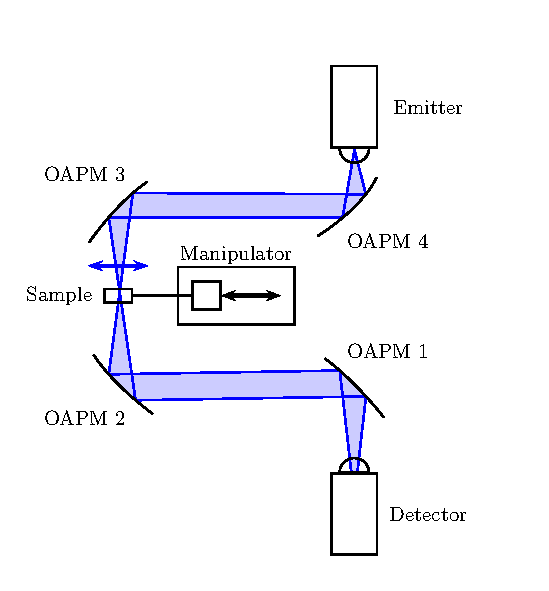
\includegraphics[width=0.45\linewidth]{images/setup/Setup-THz-TDS-HHI.pdf}}
    \qquad
    \subcaptionbox{\label{fig:2}}
        {\hspace*{-2em}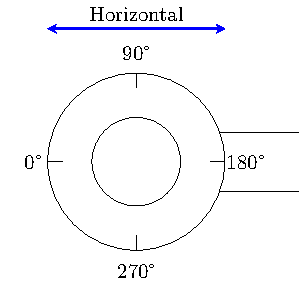
\includegraphics[width=0.45\linewidth]{images/setup/sample_mount_simple_nosample.pdf}}
    
    \caption{a): The main components of the measurement setup which consists of four off-axis parabolic mirrors, the sample mounted on a translation stage(Manipulator) as well as the emitter and detector. b): The rotational sample mount where the blue arrow indicates the horizontal direction which is also the polarization plane of the incident radiation.}
    \label{fig:3_THz-TDS-HHI}
\end{figure}

\begin{figure}[H]
    \centering
    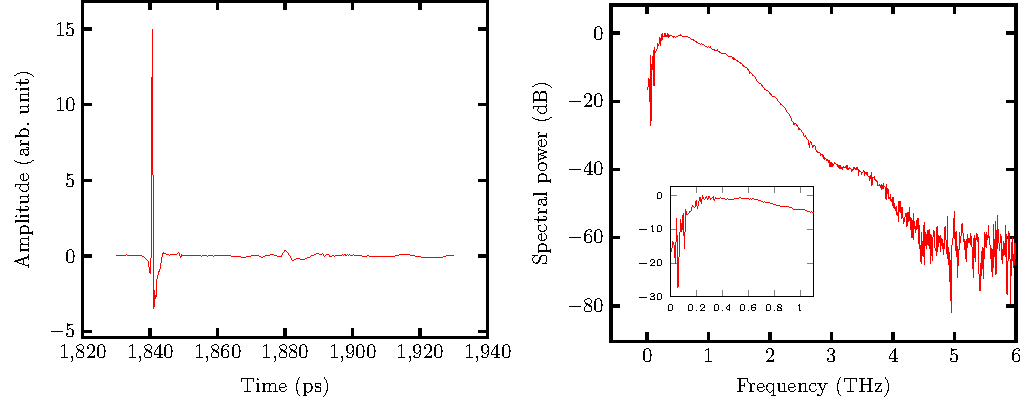
\includegraphics[scale=0.7]{images/setup/plots/pulse_example.pdf}
    \caption{Left: Example of a THz pulse from a reference measurement with 100 averages. Right: Spectrum of the pulse. The inset shows the first \SI{1}{\tera \hertz} of the spectrum with a bandwidth of around \SI{4.5}{\tera \hertz} and a signal peak at around \SI{500}{\giga \hertz}.}
    \label{fig:HHI_pulse_example}
\end{figure}

Figure \ref{fig:HHI_pulse_example} a) shows the time-domain signal from a \SI{100}{\pico \second} long reference measurement which consists of 100 averages recorded at \SI{80}{\milli \second} per trace. Figure \ref{fig:HHI_pulse_example} b) shows the spectrum of the pulse. We see that the spectrum contains frequency components up to around \SI{4.5}{\tera \hertz} with a signal peak at around \SI{500}{\giga \hertz}. Below around \SI{200}{\giga \hertz} the signal becomes quite noisy. Additionally, we see that with an average of 100 traces the dynamic range for this setup is around \SI{60}{\decibel}.

\section{THz-TDS bow-tie setup}
The second THz-TDS system we used in this work is shown in figure \ref{fig:THz_bowtie_setup}. For this system again an Er:Fiber laser with an average power of around \SI{80}{\milli \watt} is used. The laser generates \SI{90}{\femto \second} pulses with a central wavelength of \SI{1560}{\nano \meter} at a rate of \SI{100}{\mega \hertz}. The laser output is first attenuated using a \SI{3}{\decibel} attenuator and then split into two branches using a 50/50 fiber splitter; one branch is coupled directly into the emitter while the other part is coupled into free-space and subsequently guided via mirrors(M1-3) over a mechanical delay line to a fibercoupler which is connected to the detector. Therefore, one major difference of this setup compared to the previously described one is that the mechanical delay line is not enclosed in a separate container. Additionally, different from the TeraWave setup the detector and emitter in this setup are employing bow-tie antenna structures. Another difference is that an AC voltage of \SI{20}{\volt} with a frequency of \SI{6346}{\hertz} is generated and applied to the emitter module. The current signal generated by the detector module is in the \si{\nano \ampere} range, therefore to distinguish and extract it from the background noise a lock-in amplifier is used. To that extend the generated AC \SI{6346}{\hertz} bias is further used as a reference by the lock-in amplifier.

In this setup we placed the sample in between two polyethylene lenses which were used to collimate the beam. Similarly to the previous setup we determined the polarization of the THz beam using a wire grid polarizer. The measured transmittance at different angles showed that the radiation was again mostly horizontally linearly polarized which is indicated by a blue arrow in figure \ref{fig:THz_bowtie_setup}. The left subfigure of figure \ref{fig:THz_bowtie_setup} shows a reference measurement which consists of a single \SI{200}{\pico \second} trace; no averaging is performed due to the slower mechanical delay line compared to the delay line used in the TeraWave system and a single trace takes around \SI{150}{\second} to complete. The right subfigure shows the spectrum of the pulse. We see that the bandwidth of this setup is around \SI{700}{\giga \hertz} with a signal peak around \SI{200}{\giga \hertz}. We did not purge the measurement chamber with nitrogen since the beam path in this setup is not enclosed in a sealed container, this can also be seen by the existence of the water vapor absorption line around \SI{0.555}{\tera \hertz} \cite{VanExter1989}. Fortunately for this setup water vapor absorption is less a problem since the absorption of water vapor increases with frequency \cite{Series2019}. It is worth noting that the lower signal peak is useful in cases where the wavelength should be larger compared to the structural periodicity of the sample, which is what we use this setup for. 

\begin{figure}[H]
    \centering
    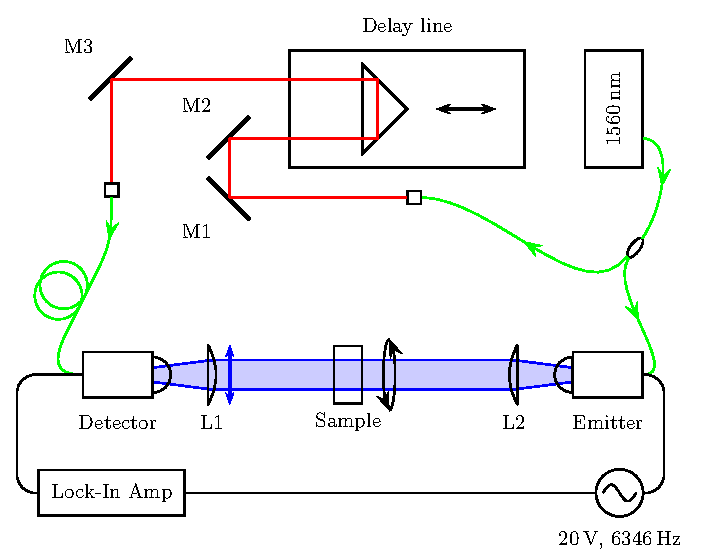
\includegraphics{images/setup/Setup-THz-TDS-Lab1.pdf}
    \caption{Schematic of the THz-TDS free-space setup. The \SI{1560}{\nano \meter} laser pulses are split into a detector branch and an emitter branch. Pulses in the detector branch are delayed by a mechanical delay line and serve as optical switches for the detector. The emitter is further modulated by a \SI{20}{\volt} \SI{6346}{\hertz} bias which is used as a reference by the lock-in amplifier to separate the detector signal from background noise. In this setup the THz beam is collimated and horizontally linearly polarized as indicated by the blue arrow.}
    \label{fig:THz_bowtie_setup}
\end{figure}

\begin{figure}[H]
    \centering
    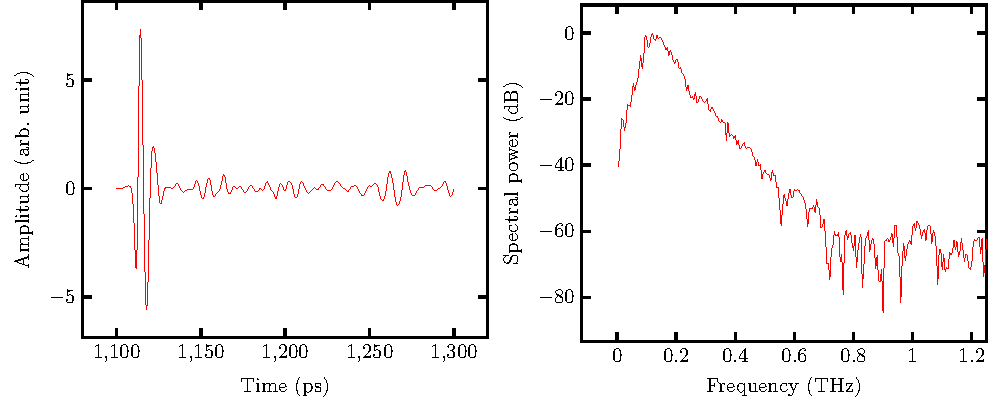
\includegraphics[scale=0.58]{images/setup/plots/pulse_example_bt.pdf}
    \caption{Left: Example of a THz pulse from a single \SI{200}{\pico \second} long reference measurement. Right: Spectrum of the pulse, which shows a bandwidth of around \SI{700}{\giga \hertz} with a signal peak around \SI{200}{\giga \hertz}}
    \label{fig:BT_pulse_example}
\end{figure}

\section{Quasi-optical GHz setup}
\label{sec:GHz_setup}
The rapid drop-off in spectral power at lower frequencies which we see for the two previously described setups show that especially at the lower end of the THz range high resolution measurements are difficult to perform with conventional THz-TDS setups. Additionally, for the characterization of form birefringent stratified structures with spatial periods in the lower millimeter range setups with higher resolution and SNR in the millimeter wavelength range are better suited. These samples were characterized by the High Frequency and Electromagnetic Fields group which is a department of the Physikalisch-Technische Bundesanstalt located near Braunschweig\footnote{\url{https://www.ptb.de/cms/en/ptb/fachabteilungen/abt2/fb-22.html}} since we do not have access to such setups; all measurements with the quasi-optical GHz setup (GHz setup) were therefore performed by this group.

For the characterization they used a free-space quasi-optical setup based on a vector network analyzer(VNA). A schematic of the setup is shown in figure \ref{fig:GHz_setup}, it mainly consists of a commercial VNA and different waveguide frequency extension unit sets. The frequency extension units allow the frequency range of the measurement to be converted into one of the following six ranges: \SIrange[range-phrase=--]{50}{75}{\giga \hertz}, \SIrange[range-phrase=--]{75}{110}{\giga \hertz}, \SIrange[range-phrase=--]{110}{170}{\giga \hertz}, \SIrange[range-phrase=--]{140}{220}{\giga \hertz}, \SIrange[range-phrase=--]{220}{325}{\giga \hertz} and from \SIrange{325}{500}{\giga \hertz}. We chose the range \SIrange{75}{110}{\giga \hertz} since it is wider than the range starting at \SI{50}{\giga \hertz} and the wavelength in this range is \SIrange{2.7}{4.0}{\milli \meter} which is still well into the \si{\milli \meter} range. 

\begin{figure}[H]
    \centering
    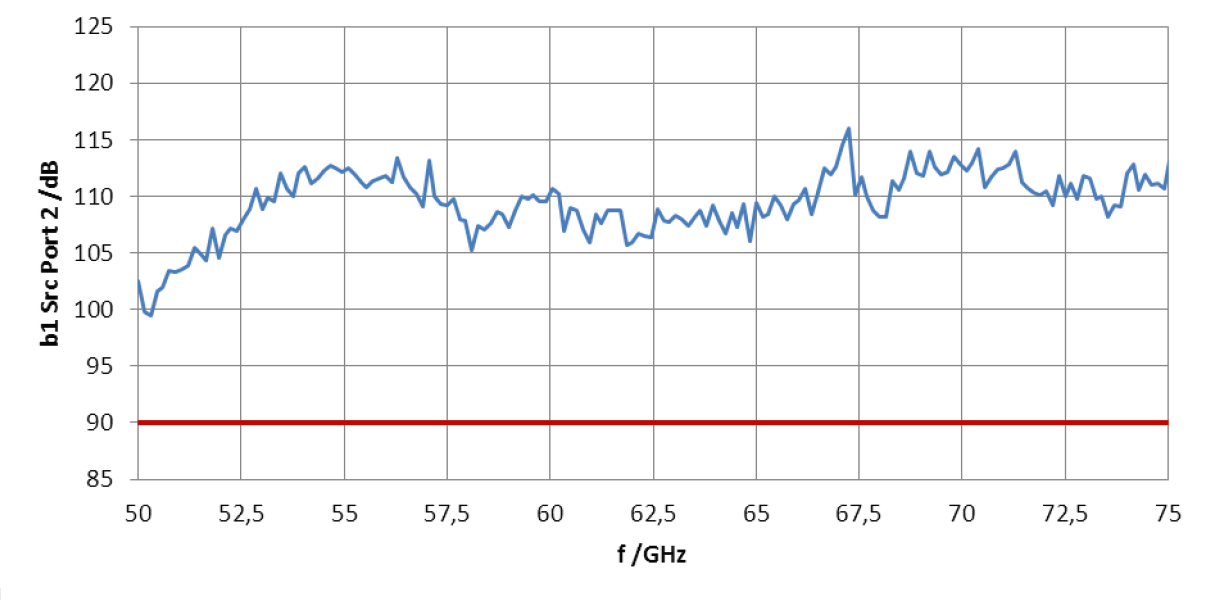
\includegraphics[scale=0.4]{images/setup/DNR.png}
    \caption{Dynamic range in dB versus frequency of the VNA combined with the \SIrange[range-phrase=--]{75}{110}{\giga \hertz} frequency extender. Source: \cite{VNADNR2013}}
    \label{fig:VNA_DNR}
\end{figure}

Furthermore, the waveguide ports of the frequency extenders are connected to two rectangular horn antennas and two OAPM are used to reduce transmission losses. It is worth noting that similarly to the PCAs, conventional horn antennas also have a linear emission pattern \cite{ShiChen2013}. With this setup we get a frequency resolution of \SI{25}{\mega \hertz} while in case of the THz-TDS systems we get a resolution of \SI{5}{\giga \hertz} for a trace length of \SI{200}{\pico \second}. Figure \ref{fig:VNA_DNR} shows the dynamic range of the VNA and selected frequency converter system. We see that compared to the THz pulses the VNA has a fairly flat spectrum \cite{VNADNR2013, Kazemipour2015}.

\begin{figure}[H]
    \centering
    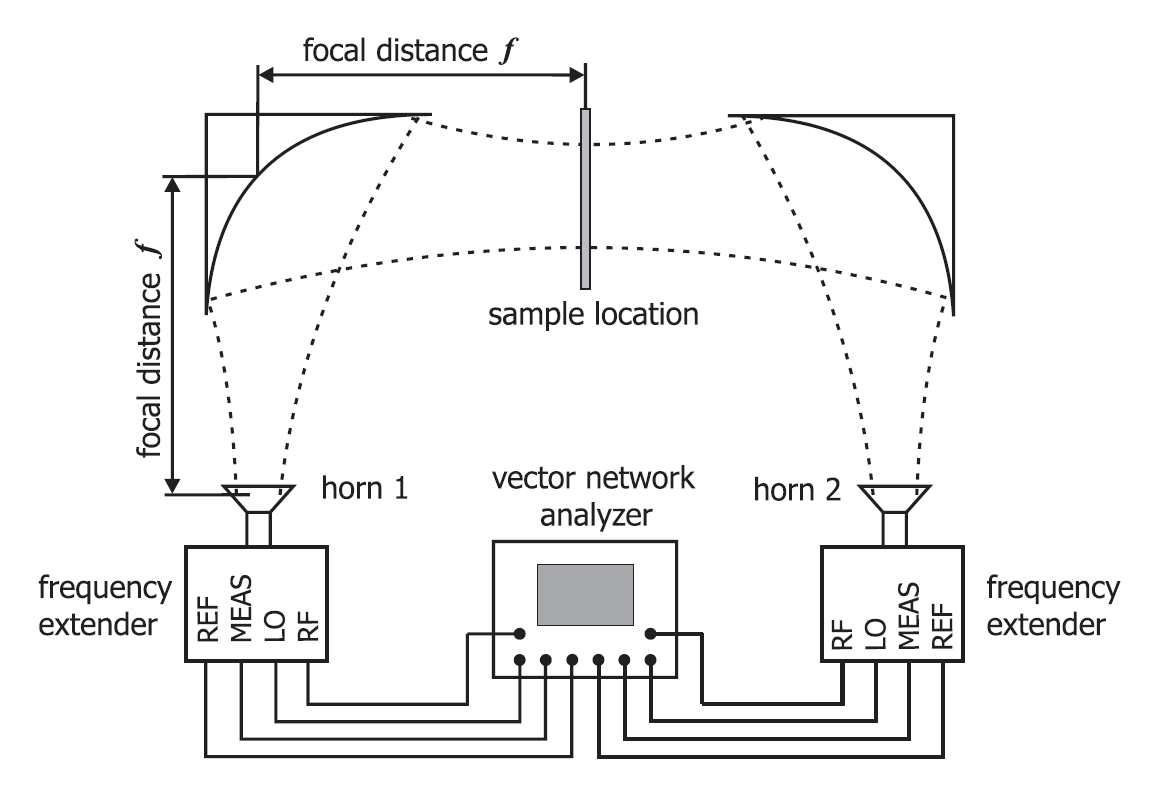
\includegraphics[scale=0.4]{images/setup/ghz.png}
    \caption{Schematic of the quasi-optical GHz setup. The vector network analyzer generates and measures the signal from which the S-parameters are obtained. A frequency extender enables the measurement to be performed from \SIrange{75}{110}{\giga \hertz}. Two OAPM reduce free-space transmission losses. Source: \cite{Kazemipour2015}}
    \label{fig:GHz_setup}
\end{figure}

The VNA measures the so called scattering parameters or S-parameters directly at each frequency. Simply put the S-parameters relate the EM-waves travelling towards and away from each antenna \cite{Caspers2012}. This means that if one considers the multiple reflections inside of the sample then they directly relate to the transmission and reflection coefficients of free space in combination with the sample. In order to extract the permittivity of the sample from the measured S-parameters a reference measurement is therefore required. The execution of the measurement and the extraction process is described in more detail in \cite{Kazemipour2015}. 
